\section{Pendule à N maillons}

Cette section aborde le cas du pendule à $N$ maillons, et plus spécifiquement le cas du pendule simple et du pendule double.

\subsection{Simple pendule}

Un simple pendule correspond à une masse $m$ (ponctuelle) attachée à l'extrémité d'un fil de longueur $l$ sans masse et inextensible qui oscille sous l'effet de la gravité.

Considérons un pendule de masse $m$, de longueur $l$, et d'angle $\theta$ par rapport à la verticale. L'équation différentielle \ref{eq:simple_pendulum} ci-dessous est obtenu par l'application du \textbf{Principe Fondamental de la Dynamique} (PFD) sur $m$.
\begin{align}
    \frac{d\varepsilon}{dt} &= 0 \\
    \varepsilon &= \varepsilon_k + \varepsilon_p \\
    \varepsilon_k &= \frac{1}{2}mv^2 \text{avec $v = l\dot{\theta}$} \\
    &\text{soit $\varepsilon_k = \frac{1}{2}ml^2\dot{\theta}^2$} \\
    &\text{et $\theta = \frac{\pi}{2}, \varepsilon_p = -mgl \cos{\theta}$} \\
    \varepsilon &= \frac{1}{2}ml^2\dot{\theta}^2 - mgl\cos{\theta} \\
    \frac{d\varepsilon}{dt} &= ml^2\dot{\theta}\ddot{\theta} + mgl \sin{\theta\dot{\theta}} \\
    &\text{d'où $\boxed{\ddot{\theta} = \frac{g}{l}\sin{\theta}}$}
    \label{eq:simple_pendulum}
\end{align}

En considérant de faibles oscillations, ainsi que le développement de $\sin$ au voisinage de zéro (premier ordre), on a alors l'équation différentielle $\ddot{\theta} = -\frac{g}{l}\sin{\theta}$. La résolution de celle-ci se fait par l'utilisation des méthodes évoquées précédemment, et plus spécifiquement la méthode de \textbf{Runge-Kutta d'ordre 4} dans notre cas.

On considère le vecteur 
\vspace{4.00mm}

\begin{equation}
    X(t) = \begin{pmatrix} \theta(t) \\ \dot{\theta}(t) \end{pmatrix}
\end{equation}
, d'où 
\begin{equation}
    X'(t) = \begin{pmatrix} \ddot{\theta}(t) \\ \frac{g}{l}\sin{\theta(t)} \end{pmatrix} = f(t, X(t))
    \label{eq:dif_simple_pendulum}
\end{equation}


Comme expliqué précédemment, nous avons utilisé la méthode de \textbf{Runge-Kutta d'ordre 4} pour obtenir la variation de l'angle $\theta$ en fonction du temps (Figure \ref{fig:var_theta}). Ensuite, nous avons réalisé le tracé de la variation de la fréquence en fonction de l'angle initial $\theta_0$ (Figure \ref{fig:var_freq}), tout en utilisant la méthode \textbf{Runge-Kutta d'ordre 4}. En outre, on remarque que pour un petit angle $\theta$, la fréquence s'approche de $\frac{\sqrt{g}}{2*\pi*\sqrt{l}}$

\begin{minipage}[c]{.46\linewidth}
    \centering
    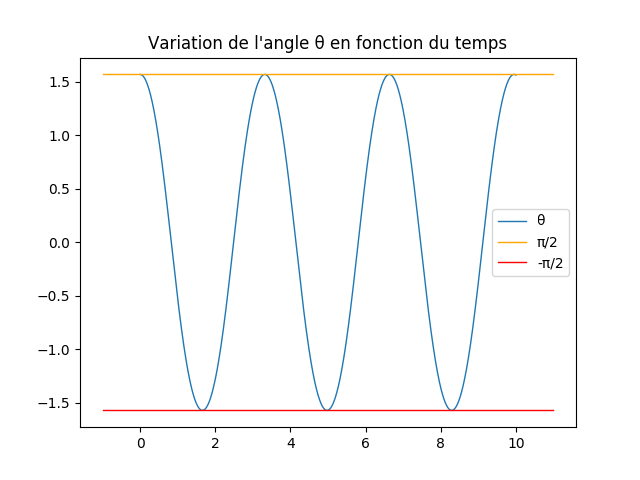
\includegraphics[width=\linewidth]{images/var_theta.png}
    \captionsetup{type=figure}\caption{Variation de l'angle $\theta$ en fonction du temps (Résolution de l'équation différentielle \ref{eq:dif_simple_pendulum} pour $m = 1kg$, $l = 1m$, $g = 9.81m/s^2$) et $\theta_0 = \frac{\pi}{2}$.}
    \label{fig:var_theta}
\end{minipage}
\hfill%
\begin{minipage}[c]{.46\linewidth}
    \centering
    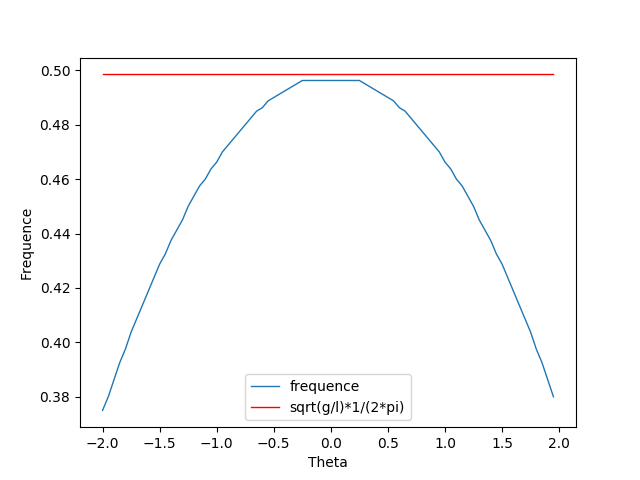
\includegraphics[width=\linewidth]{images/var_freq.png}
    \captionsetup{type=figure}\caption{Variation de la fréquence d'oscillation en fonction de l'angle initial $\theta_0$ (pour $m = 1kg$, $l = 1m$, $g = 9.81m/s^2$).}
    \label{fig:var_freq}
\end{minipage}


\subsection{Double pendule}
Le double pendule consiste en l'ajout d'un second pendule simple de longueur $l_2$ et de masse $m_2$ au niveau de la masse du premier pendule.

Ainsi, on utilise la même méthode que précédemment pour résoudre le système. On considère le vecteur : 

\vspace{4.00mm}
\begin{equation}
    X(t) = \begin{pmatrix} \theta_1(t) \\ \dot{\theta_1}(t) \\ \theta_2(t) \\ \dot{\theta_2}(t) \end{pmatrix}
\end{equation}
, d'où 
\begin{equation}
    X'(t) = \begin{pmatrix} \dot{\theta_1}(t) \\ \frac{-g(2m_1 + m_2)\sin{\theta_1(t)}-m_2g\sin(\theta_1(t)-2\theta_2(t))-2\sin(\theta_1(t) - \theta_2(t))m_2(\omega^{2}_2L_2+\omega^{2}_1L_1\cos(\theta_1(t) - \theta_2(t)))}{L_1(2m_1+m_2-m_2\cos(2\theta_1(t) - 2 \theta_2(t)))} \\ \dot{\theta_2}(t) \\ \frac{2\sin(\theta_1(t) - \theta_2(t))(\omega^{2}_1L_1(m_1+m_2)+g(m_1 + m_2)\cos{\theta_1(t)} + \omega^{2}_2L_2m_2\cos(\theta_1(t) - \theta_2(t)))}{L_2(2m_1+m_2-m_2\cos(2\theta_1(t) - 2 \theta_2(t)))} \end{pmatrix}
\end{equation}

Ainsi, nous pouvons simuler la trajectoire de l'extrémité du pendule à deux maillons en fonction du temps tel que montré sur la figure \ref{fig:trace_double_pendulum}. On remarque également sur cette figure, que la légère variation de l'angle $\theta_1$ ou $\theta_2$ provoque de grand changement sur la trajectoire. Ainsi, cela démontre la dépendance du système aux conditions initiales. Ce comportement est normal, car inhérent aux systèmes chaotiques dont fait parti le double pendule (du fait des deux équations différentielles liées).

\begin{minipage}[c]{.46\linewidth}
    \centering
    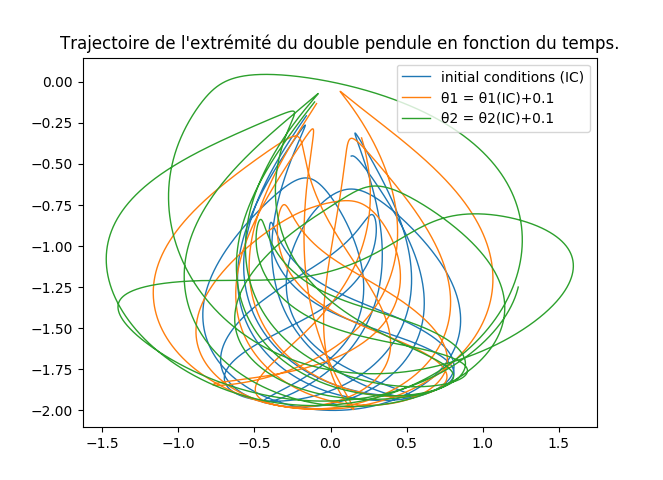
\includegraphics[width=\linewidth]{images/trace_pendule.png}
    \captionsetup{type=figure}\caption{Conditions initiales : $m_1 = m_2 = 1kg$, $l_1 = l_2 = 1 m$, $g = 9.81m/s^2$}
    \label{fig:trace_double_pendulum}
\end{minipage}
\hfill%
\begin{minipage}[c]{.46\linewidth}
    \centering
    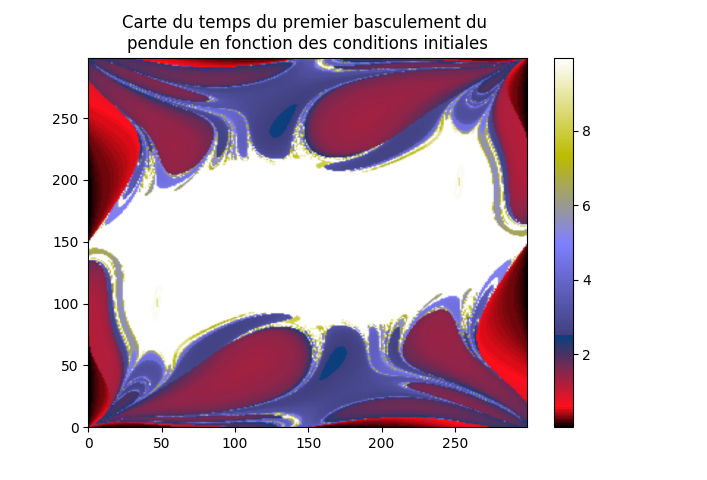
\includegraphics[width=\linewidth]{images/map_time.png}
    \captionsetup{type=figure}\caption{Conditions initiales : $m_1 = m_2 = 1kg$, $l_1 = l_2 = 1 m$, $g = 9.81m/s^2$) sur une période de $10$ secondes}
    \label{fig:map_time}
\end{minipage}
\vspace{4.00mm}

Enfin, un autre moyen permettant de mettre en avant les propriétés du système consistait en la création d'une carte du temps du premier basculement du pendule en fonction du temps (Figure \ref{fig:map_time}). Par temps de basculement, nous entendons le temps nécessaire pour que l'angle $\theta_1$ du premier pendule ou l'angle $\theta_2$ du second pendule dépasse $\pi$. De part les variations de couleurs, on remarque rapidement qu'il devient très compliqué de prévoir les mouvements du double pendule. En effet, pour un changement minime de $\theta$, le temps de basculement peut se produire bien plus tardivement, voir jamais.


\section{Conclusion}
Pour conclure, ce projet a mis en avant l'efficacité des méthodes de résolution d'équations différentielles ordinaires pour certaines applications. Nous avons également mesuré l'importance de la généricité du code en raison des dimensions différentes associées aux fonctions de ces équations. Ensuite, nous avons abordé deux applications différentes, mais avoir le temps de toutes les traitées aurait pu donner un plus large aperçu de la puissance de résolution liée aux méthodes implémentées. Enfin, nous avons été en mesure de constater la difficulté de prédire certains comportements relatifs aux systèmes chaotiques, dus à leurs dépendances aux conditions initiales.